% Source for docs/static/img/comparator-pairs.svg. Rebuild from the repository root:
%   pdflatex -output-directory=/tmp docs/scripts/comparator-pairs.tex
%   pdf2svg /tmp/comparator-pairs.pdf docs/static/img/comparator-pairs.svg
%   python3 docs/scripts/prepare_rollout_svgs.py
% Keep the stage boundaries in prepare_rollout_svgs.py in sync with the row positions.
% Shared preamble for the CoMLRL training-flow diagrams. Paste it verbatim at the
% top of every diagram so each .tex stays standalone.
\documentclass[tikz,border=3pt]{standalone}
\usepackage{amsmath,amssymb,bm}
\usetikzlibrary{arrows.meta,positioning,calc,fit}

% Only these paints have dark-theme mappings (assets/_diagram-theme.scss).
\colorlet{agentA}{red!80!black}     % agent 1: policy, prompts, responses, loss
\colorlet{agentB}{blue!80!black}    % agent 2
\colorlet{learned}{orange!80!black} % learned evaluators: critic, reward model
\colorlet{update}{green!50!black}   % gradients and parameter updates
% Joint or shared quantities are black. Gray = black with fill opacity.

\tikzset{
  >={Stealth[length=3.2pt,width=3pt]},
  box/.style={draw, line width=1pt, inner sep=2.5pt, minimum height=13pt},
  policy/.style={box, rounded corners=3pt, minimum width=30pt},
  flow/.style={->, line width=.8pt},
  note/.style={font=\scriptsize, align=left},
  label/.style={anchor=west, font=\footnotesize},
}

% Iterative comparator: the comparator's source, index-aligned samples, task-reward
% comparisons (either side can win) and the iteration's pairs D^(nu).
% Rows are animation stages; avoid \frac and \_ (their rules animate as edges).
\begin{document}
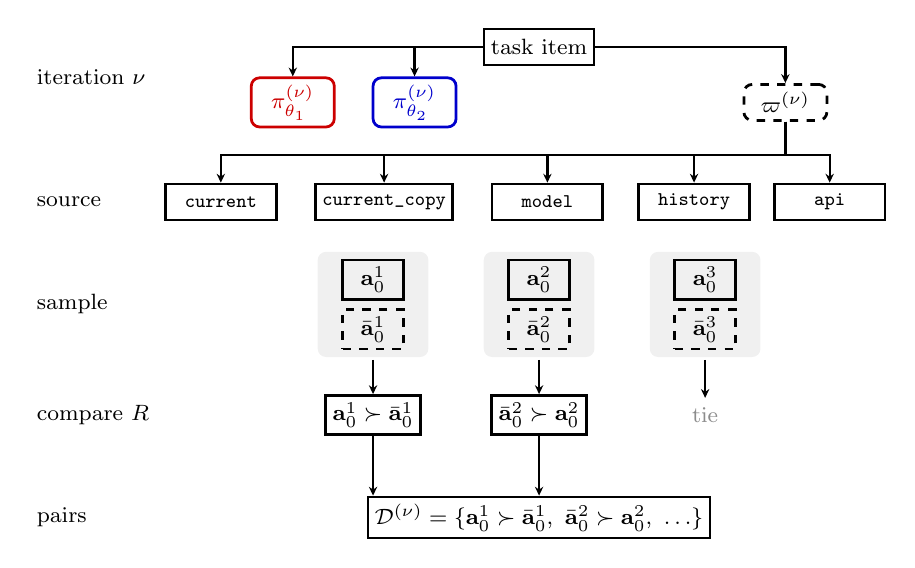
\begin{tikzpicture}[x=1pt, y=1pt, font=\footnotesize]
  \def\ka{125} \def\kb{185} \def\kc{245} % candidate index columns
  \tikzset{cand/.style={box, minimum width=22pt}}

  % Stage 0: iteration nu, the current actors and the comparator on one task item.
  \node[label] at (0,-11) {iteration $\nu$};
  \node[box] (x) at (185,0) {task item};
  \node[policy, agentA] (p1) at (96,-20) {$\pi^{(\nu)}_{\theta_1}$};
  \node[policy, agentB] (p2) at (140,-20) {$\pi^{(\nu)}_{\theta_2}$};
  \node[policy, dashed] (c) at (274,-20) {$\varpi^{(\nu)}$};
  \draw[flow] (x.west) -| (p1.north);
  \draw[flow] (x.west) -| (p2.north);
  \draw[flow] (x.east) -| (c.north);

  % Stage 1: the comparator's source.
  \node[label] at (0,-56) {source};
  \foreach \n/\x/\t in {s1/70/current, s2/129/current\char95copy, s3/188/model,
                        s4/241/history, s5/290/api} {
    \node[box, minimum width=40pt, font=\scriptsize\ttfamily] (\n) at (\x,-56) {\t};
    \draw[flow] (c.south) |- ++(0,-12) -| (\n.north);
  }

  % Stage 2: both sides sample; candidates with the same index k are compared.
  \node[label] at (0,-93) {sample};
  \foreach \x/\k in {\ka/1,\kb/2,\kc/3} {
    \fill[black, fill opacity=.06, rounded corners=3pt] (\x-20,-74) rectangle (\x+20,-112);
    \node[cand] at (\x,-84) {$\mathbf{a}^{\k}_0$};
    \node[cand, dashed] at (\x,-102) {$\bar{\mathbf{a}}^{\k}_0$};
  }

  % Stage 3: the task reward decides each comparison; ties are dropped.
  \node[label] at (0,-133) {compare $R$};
  \node[box] (w1) at (\ka,-133) {$\mathbf{a}^1_0\succ\bar{\mathbf{a}}^1_0$};
  \node[box] (w2) at (\kb,-133) {$\bar{\mathbf{a}}^2_0\succ\mathbf{a}^2_0$};
  \node[opacity=.45] (w3) at (\kc,-133) {tie};
  \foreach \x/\w in {\ka/w1,\kb/w2,\kc/w3} \draw[flow] (\x,-113) -- (\w.north);

  % Stage 4: the iteration's preference pairs.
  \node[label] at (0,-170) {pairs};
  \node[box] (D) at (185,-170)
    {$\mathcal{D}^{(\nu)}=\{\mathbf{a}^1_0\succ\bar{\mathbf{a}}^1_0,\ \bar{\mathbf{a}}^2_0\succ\mathbf{a}^2_0,\ \ldots\}$};
  \draw[flow] (w1.south) -- (\ka,0 |- D.north);
  \draw[flow] (w2.south) -- (\kb,0 |- D.north);
\end{tikzpicture}
\end{document}
